\section{Introduction}

This document is to summarise our experiments attempted to bias the seeding procedure of CC2538\cite{CC2538_Manual}.

The greatest difficulty is that details of how the seeding is done is not disclosed by the released documents from TI. The only descriptions in CC2538 User Manual are:
\begin{quote}
...For the CC2538, when a random value is required, writing the SOC\_ADC\_RNDL register with random bits from the IF\_ADC in the RF receive path seeds the LFSR. To use this seeding method, first power on the radio. The radio must be placed in the infinite RX state to avoid possible sync detect in the RX state.The random bits from the IF\_ADC are read from the LSB position of the RF register RFCORE\_XREG\_RFRND. These bits should be concatenated over time to form the bytes needed for the RNG seed... This cannot be done while the radio is in use for normal tasks... (Section 16.2.2, CC2538 User Manual)

...The RF Core can generate random bits. The chip should be in RX when generation of random bits is required. One must also make sure that the chip has been in RX long enough for the transients to have died out. A convenient way to do this is to wait for the RSSI-valid signal to go high. Single random bits from either the I or Q channel can be read from the RFRND register... (Section 23.12, CC2538 User Manual)
\end{quote}

\Cref{CC2538_RFRND} shows the description of the crucial RFRND register in its manual.

\begin{figure}
\center
\caption{Description of RFRND from CC2538 User Manual}
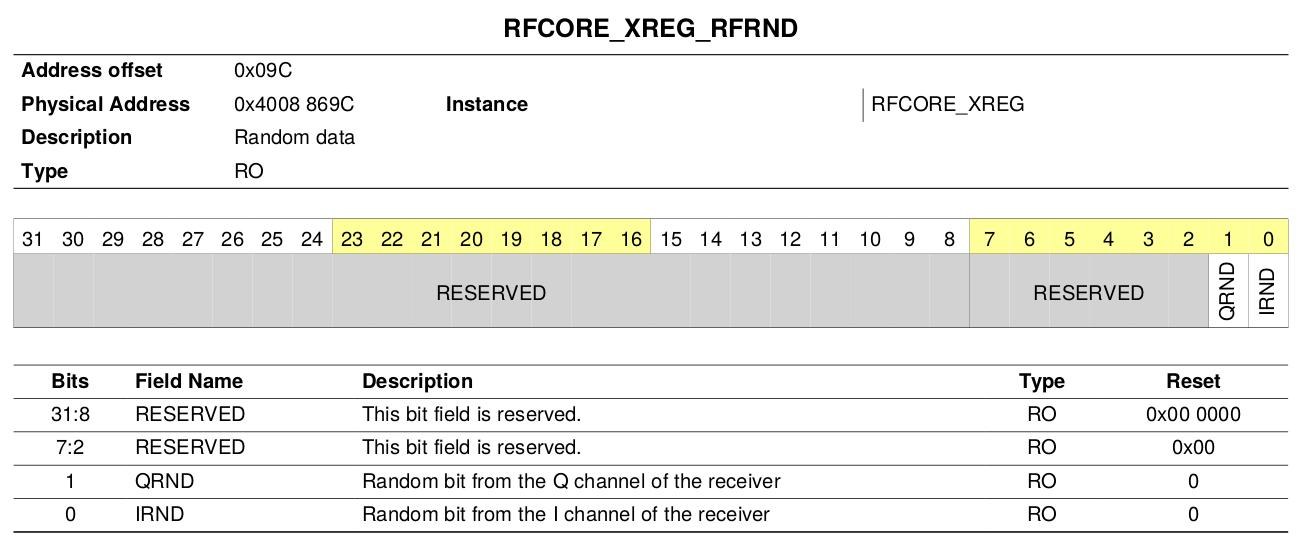
\includegraphics[width=\linewidth]{./figures/CC2538_RFRND.png}
\label{CC2538_RFRND}
\end{figure}

What we learned from the above descriptions are:
\begin{enumerate}
\item The random bits are derived from the IQ channels of IF\_ADC in the receive path, one bit at once, accessed through RFRND register.
\item The random bits are not available until the transients of IF\_ADC has died out.
\end{enumerate}

The above information seems to be good enough for developers to write drivers for this device. But from a security perspective, this method shed a light that the seed can be potentially affected by manipulating IF\_ADC through radio signals. However, there are several critical question that is not clear in the released documents:
\begin{enumerate}
\item How does IF\_ADC converts to a random bit?
\item Why infinite RX state is required?
\item Does RSSI play a role in the procedure? If yes, how?
\item What are the electronic characteristics? Including what is the IF, sample rate, etc.
\end{enumerate}

Without knowing the answers to these questions, we took two approaches to carry on the research:
\begin{enumerate}
\item Searching for related contents in the documents of product in the same series as they may shared the same design.
\item Black box experiments.
\end{enumerate}

CAUTION: Since the statements in this report are based on empirical document studies and black box experiments; thus they might not be accurate. As of writing this report, we have not yet successfully biased the seed.

\section{Related Documents Study}

CC2538, launched in May 2013, is not the first product that adopts the design of using RF to seed its PRNG, which is a 16-bit CRC16 LSFR register. The same design can trace back to one of its predecessor CC2430\cite{CC2430_Manual}, launched in 2007,  where a RNG failure has been explained by this blog\cite{CC2430Fail}.

In CC2430 User Manual, we found the following instructions:
\begin{quote}
...When a true random value is required, the LFSR should be seeded by writing RNDL with random values from the IF\_ADC in the RF receive path. To use this seeding method, the radio must first be powered on by enabling voltage regulator as described in section 15.1. The radio should be placed in infinite TX\footnote{This is actually a typo. The RF needs to be in infinite RX state to use this seeding method.} state, to avoid possible sync detect in RX state. The random values from the IF\_ADC are read from the RF registers ADCTSTH and ADCTSTL (see page 196). The values read are used as the seed values to be written to the RNDL register as described above. Note that this can not be done while radio is in use for normal tasks... (Section 13.11.2.2, CC2430 User Manual)
\end{quote}

We can see that CC2538 User Manual basically inherited the same sentences, except that the seed is instead read from different registers, ADCTSTH and ADCTSTL. \Cref{CC2430_ADCTST} shows the detailed description of these registers in its manual.

\begin{figure}
\center
\caption{Description of ADCTSTH and ADCTSTL from CC2430 User Manual}
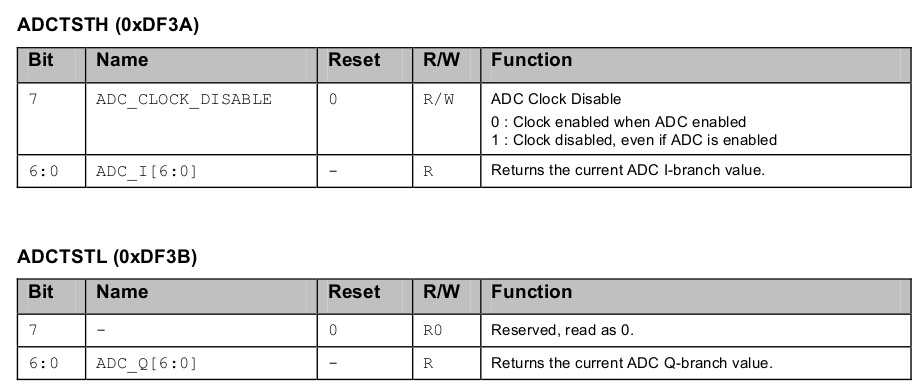
\includegraphics[width=\linewidth]{./figures/CC2430_ADCTST.png}
\label{CC2430_ADCTST}
\end{figure}

Comparing to CC2538, CC2430 User Manual explains that the ADCs have resolution of 7-bits and one of their values is suggested to be directly used as the random seed. One thing might be worthy pointing out is that the entropy test in the blog post\cite{CC2430Fail} may have incorrectly interpreted these 7-bits readings as a byte, even though it does not change the fact that such seed is strongly biased.

CC2430 also disclosed more details about its RF. \Cref{CC2430_RF} provides an overview of its RF design, which is relatively classic. We can see that the random seed from IF\_ADC is indeed the output of mixer after band pass filter and AGC, where LO is implemented by the Frequency Synthesiser.

\begin{figure}
\center
\caption{Radio and Demodulator of CC2430 from CC2430 User Manual}
\begin{subfigure}
%	\subcaption{Block Diagram of Radio Module from CC2430 User Manual}
	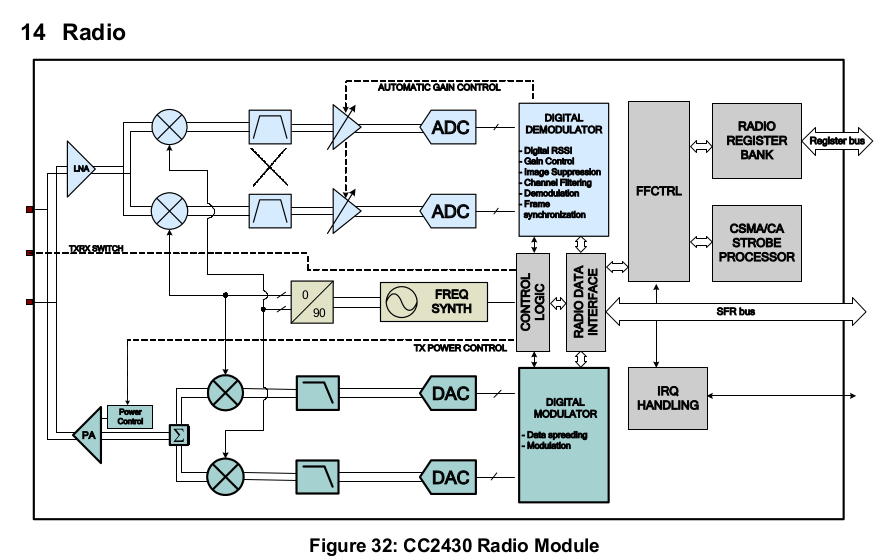
\includegraphics[width=\linewidth]{./figures/CC2430_Radio.png}
\end{subfigure}

\begin{subfigure}
%	\subcaption{Block Diagram of Demodulator from CC2430 User Manual}
	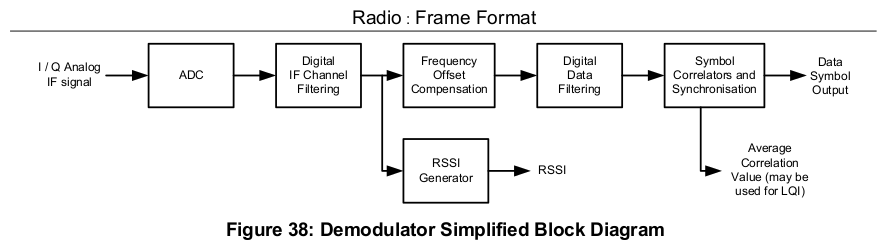
\includegraphics[width=\linewidth]{./figures/CC2430_Demodulator.png}
\end{subfigure}
\label{CC2430_RF}
\end{figure}

The CC253X and CC2540/41 series\cite{CC253X_Manual} is another sibling of CC2538 launched in April 2009. This series also inherited the similar RNG design from CC2430, using a CRC16 register as PRNG seeded by IF\_ADC.

\begin{quote}
...For the CC253x, when a random value is required, the LFSR should be seeded by writing RNDL with random bits from the IF\_ADC in the RF receive path. To use this seeding method, the radio must first be powered on. The radio should be placed in the infinite RX state to avoid possible sync detect in the RX state. The random bits from the IF\_ADC are read from the least-significant bit position of the RF register RFRND. These bits should be concatenated over time to form the bytes needed for the random-number-
generator seed... (Section 14.2.2, CC253X, CC2540/41 User Manual)
\end{quote}

\Cref{CC253X_RFRND} shows the RFRND register for CC253X.

\begin{figure}
\center
\caption{Description of RFRND from CC253X, CC2540/41 User Manual}
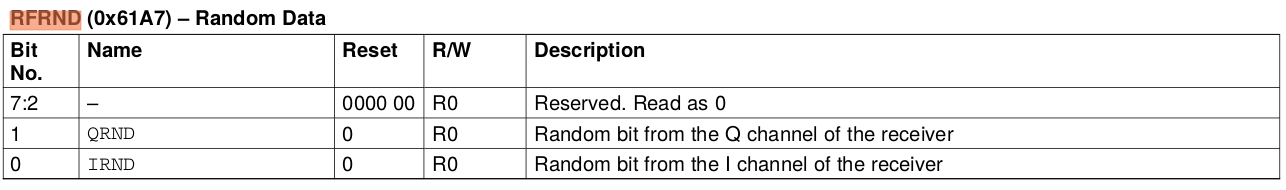
\includegraphics[width=\linewidth]{./figures/CC253X_RFRND.png}
\label{CC253X_RFRND}
\end{figure}

Further inspecting the documents, we realised that as both CC253X and CC2538 reported exactly identical seeding result, as shown in \Cref{CC2538_CC253X_SeedComparison}.

\begin{figure}
\center
\caption{Seeding Result for CC253X and CC2538}
\begin{subfigure}
	\subcaption{Seeding Result from CC253X,CC2540/41 User Manual}
	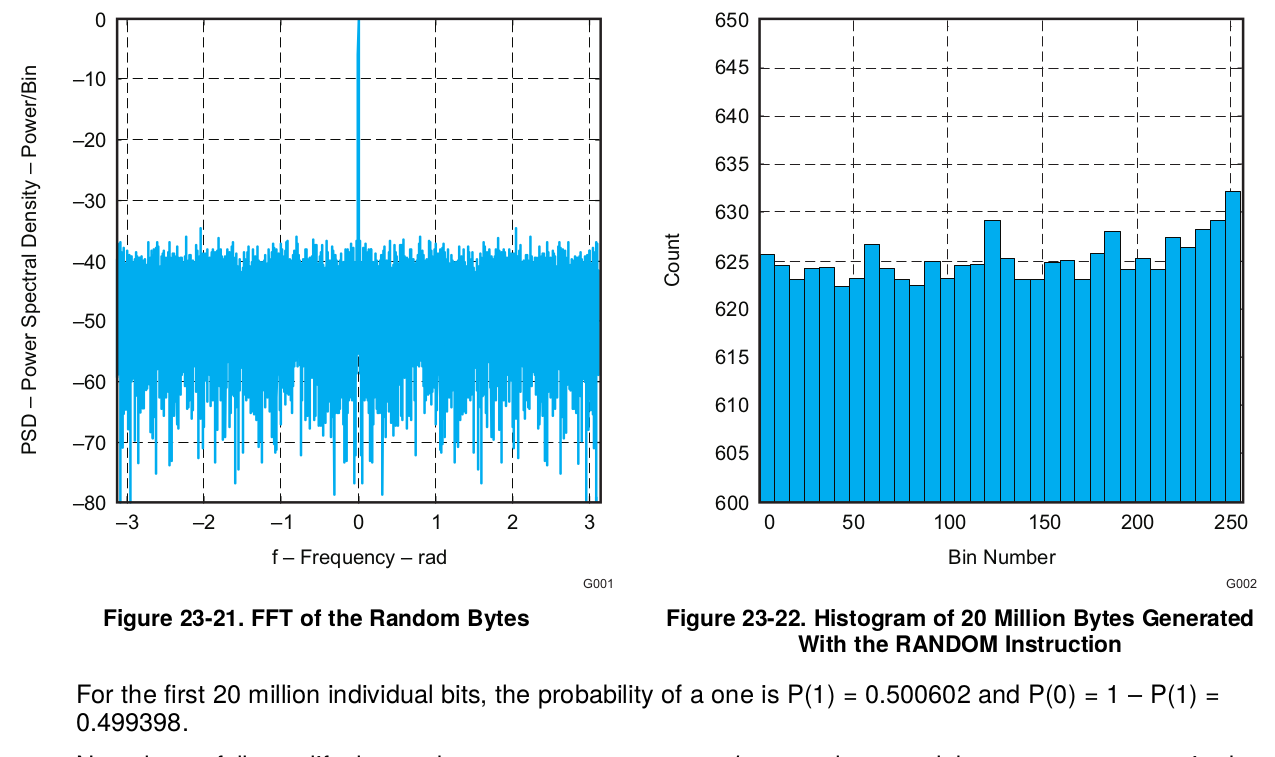
\includegraphics[width=\linewidth]{./figures/CC253X_Seed.png}
\end{subfigure}

\begin{subfigure}
	\subcaption{Seeding Result from CC2538 User Manual}
	\begin{subfigure}
	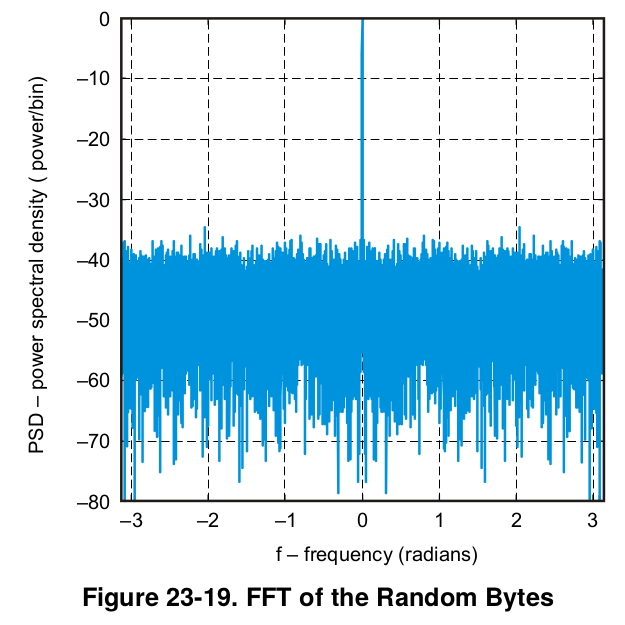
\includegraphics[width=0.5\linewidth]{./figures/CC2538_Seed1.png}
	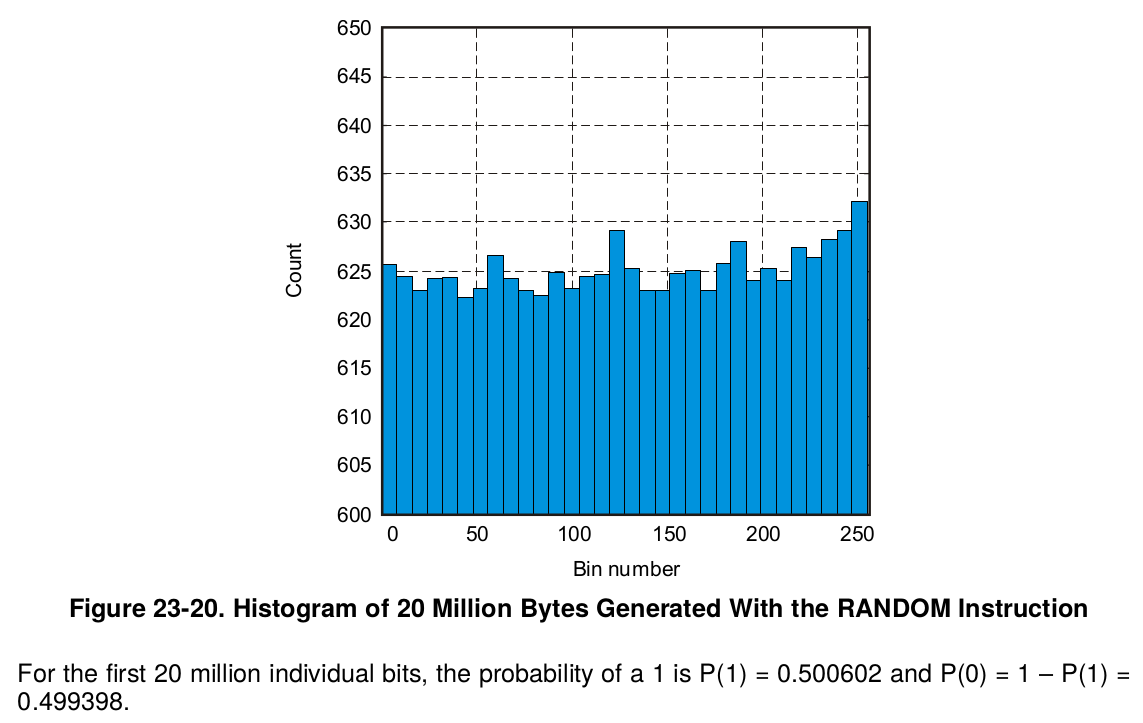
\includegraphics[width=0.9\linewidth]{./figures/CC2538_Seed2.png}
	\end{subfigure}
\end{subfigure}
\label{CC2538_CC253X_SeedComparison}
\end{figure}

However, either CC253X and CC2538 explained how IF\_ADC is translated to the output of RFRND. However, we found the following statement in the instructions for CC2541 running in proprietary mode:
\begin{quote}
...For seeding the pseudo-random number generator and for tasks where higher entropy of the random numbers is needed, the radio can be used as a true-random generator. The register RFRND provides access to the least-significant bits of the radio ADC, which is random when noise is received.... (Section 25.10, CC253X, CC2540/41 User Manual)
\end{quote}

This instruction explicitly explains that RFRND actually reads the least significant bit of IF\_ADC.

Given the similarities of these SoCs, we suspect RFRND in CC2538 is also  the least significant bit from its IF\_ADC.

In summary, we make the following assumptions about the RFRND implementation of CC2538:
\begin{enumerate}
\item RFRND is implemented as the least significant bit of IF\_ADC as of CC2541.
\item CC2538 has a similar circuit design of CC2420.
\item CC2538 has exactly the same RF of CC253X.
\end{enumerate}

\section{Black Box Experiments}

\section{Theoretic Method of Seed Biasing}
